\chapter{Methodology}\label{Ch:3}
	
\section{Design of \ac{blue}}\label{sec:Introduction3}
\subsection{Introduction to \ac{blue}}
The idea for the \ac{blue} was brought about to start designing the next rehabilitation robot that will be based on the newest technology available in rehabilitation robotics. This sprung a need for a new review on the state of robots, and in particular bilateral rehabilitation robots. This was recently done and the last proper review paper on bilateral robots was in 2016.\\
The main idea was to design a locally made version of the \acf{biadler} \cite{Christopher2014,Johnson2011a,Lott2016}, which was built to test the idea of using a robot to train specific tasks that patients lost the ability to be do because of their stroke such as: drinking, eating, reach and grabbing an object. Other researchers have done work on this topic and it led to various bilateral robots such as the \acf{ulexo} \cite{Perry2007}, the \acf{bias} system \cite{Johnson2011b}, \acf{mime} and \acf{arcmime} \cite{Burgar2011,Lum2002,Lum2005,Mahoney2003}, the \acf{bmt} \cite{Hung2019b}, the bimanual lifting rehabilitator \cite{Lum1995} and others more.

\subsection{Objectives and Specifications of \ac{blue}}
Based off the aim of the project, a list of specification can be determined for use for designing the robot. The overall desired specifications are:
\begin{itemize}%blue old specifications
	\item  3D workspace
	\item Have a suitable control method for bilateral robots
	\item similar design to the Bi-ADLER for simplicity
	\label{item:specs}
\end{itemize}
The \ac{blue} is aimed to be a Bilateral option for patient to use between it and the unilateral robot \ac{pulsr}, and to be able to quantify the difference in recovery rate between unilateral and bilateral robots.\\
%maybe remove
Due to Time Constraints, the Objectives have been simplified to 
\begin{itemize}%blue new specifications
	\item Now to be a planar bilateral robot.
	\item use a mirror-image control, as it is the suitable method for this study.
	\item Use the \ac{pulsr} arm structure as it has been analysed before.
\end{itemize}
\subsection{Design Process for \ac{blue}}
The design plan of this robot have been listed in \ref{item:specs}, and that is what is implemented in Figure \ref{fig:blue1},where the arm shown there is designed similar to the \ac{biadler} from \cite{Johnson2011}.
Simplifying the Design to suit the materials available in Nigeria, Figure \ref{fig:blue2} shows the end result of the considerations. After implementing the constraints listed above the final design for the robot is shown in Figure \ref{fig:blue3}.\\
There is also a small scare version that has been made for the purpose of demonstration of the concept shown in Figure \ref{fig:bluepres}, using parts from \ac{pulsr}2.0 and motors from \ac{pulsr}3.0 to produce the system shown in Figure \ref{fig:bluepres}.

\begin{figure}[p]%blue design 1
	\centering
	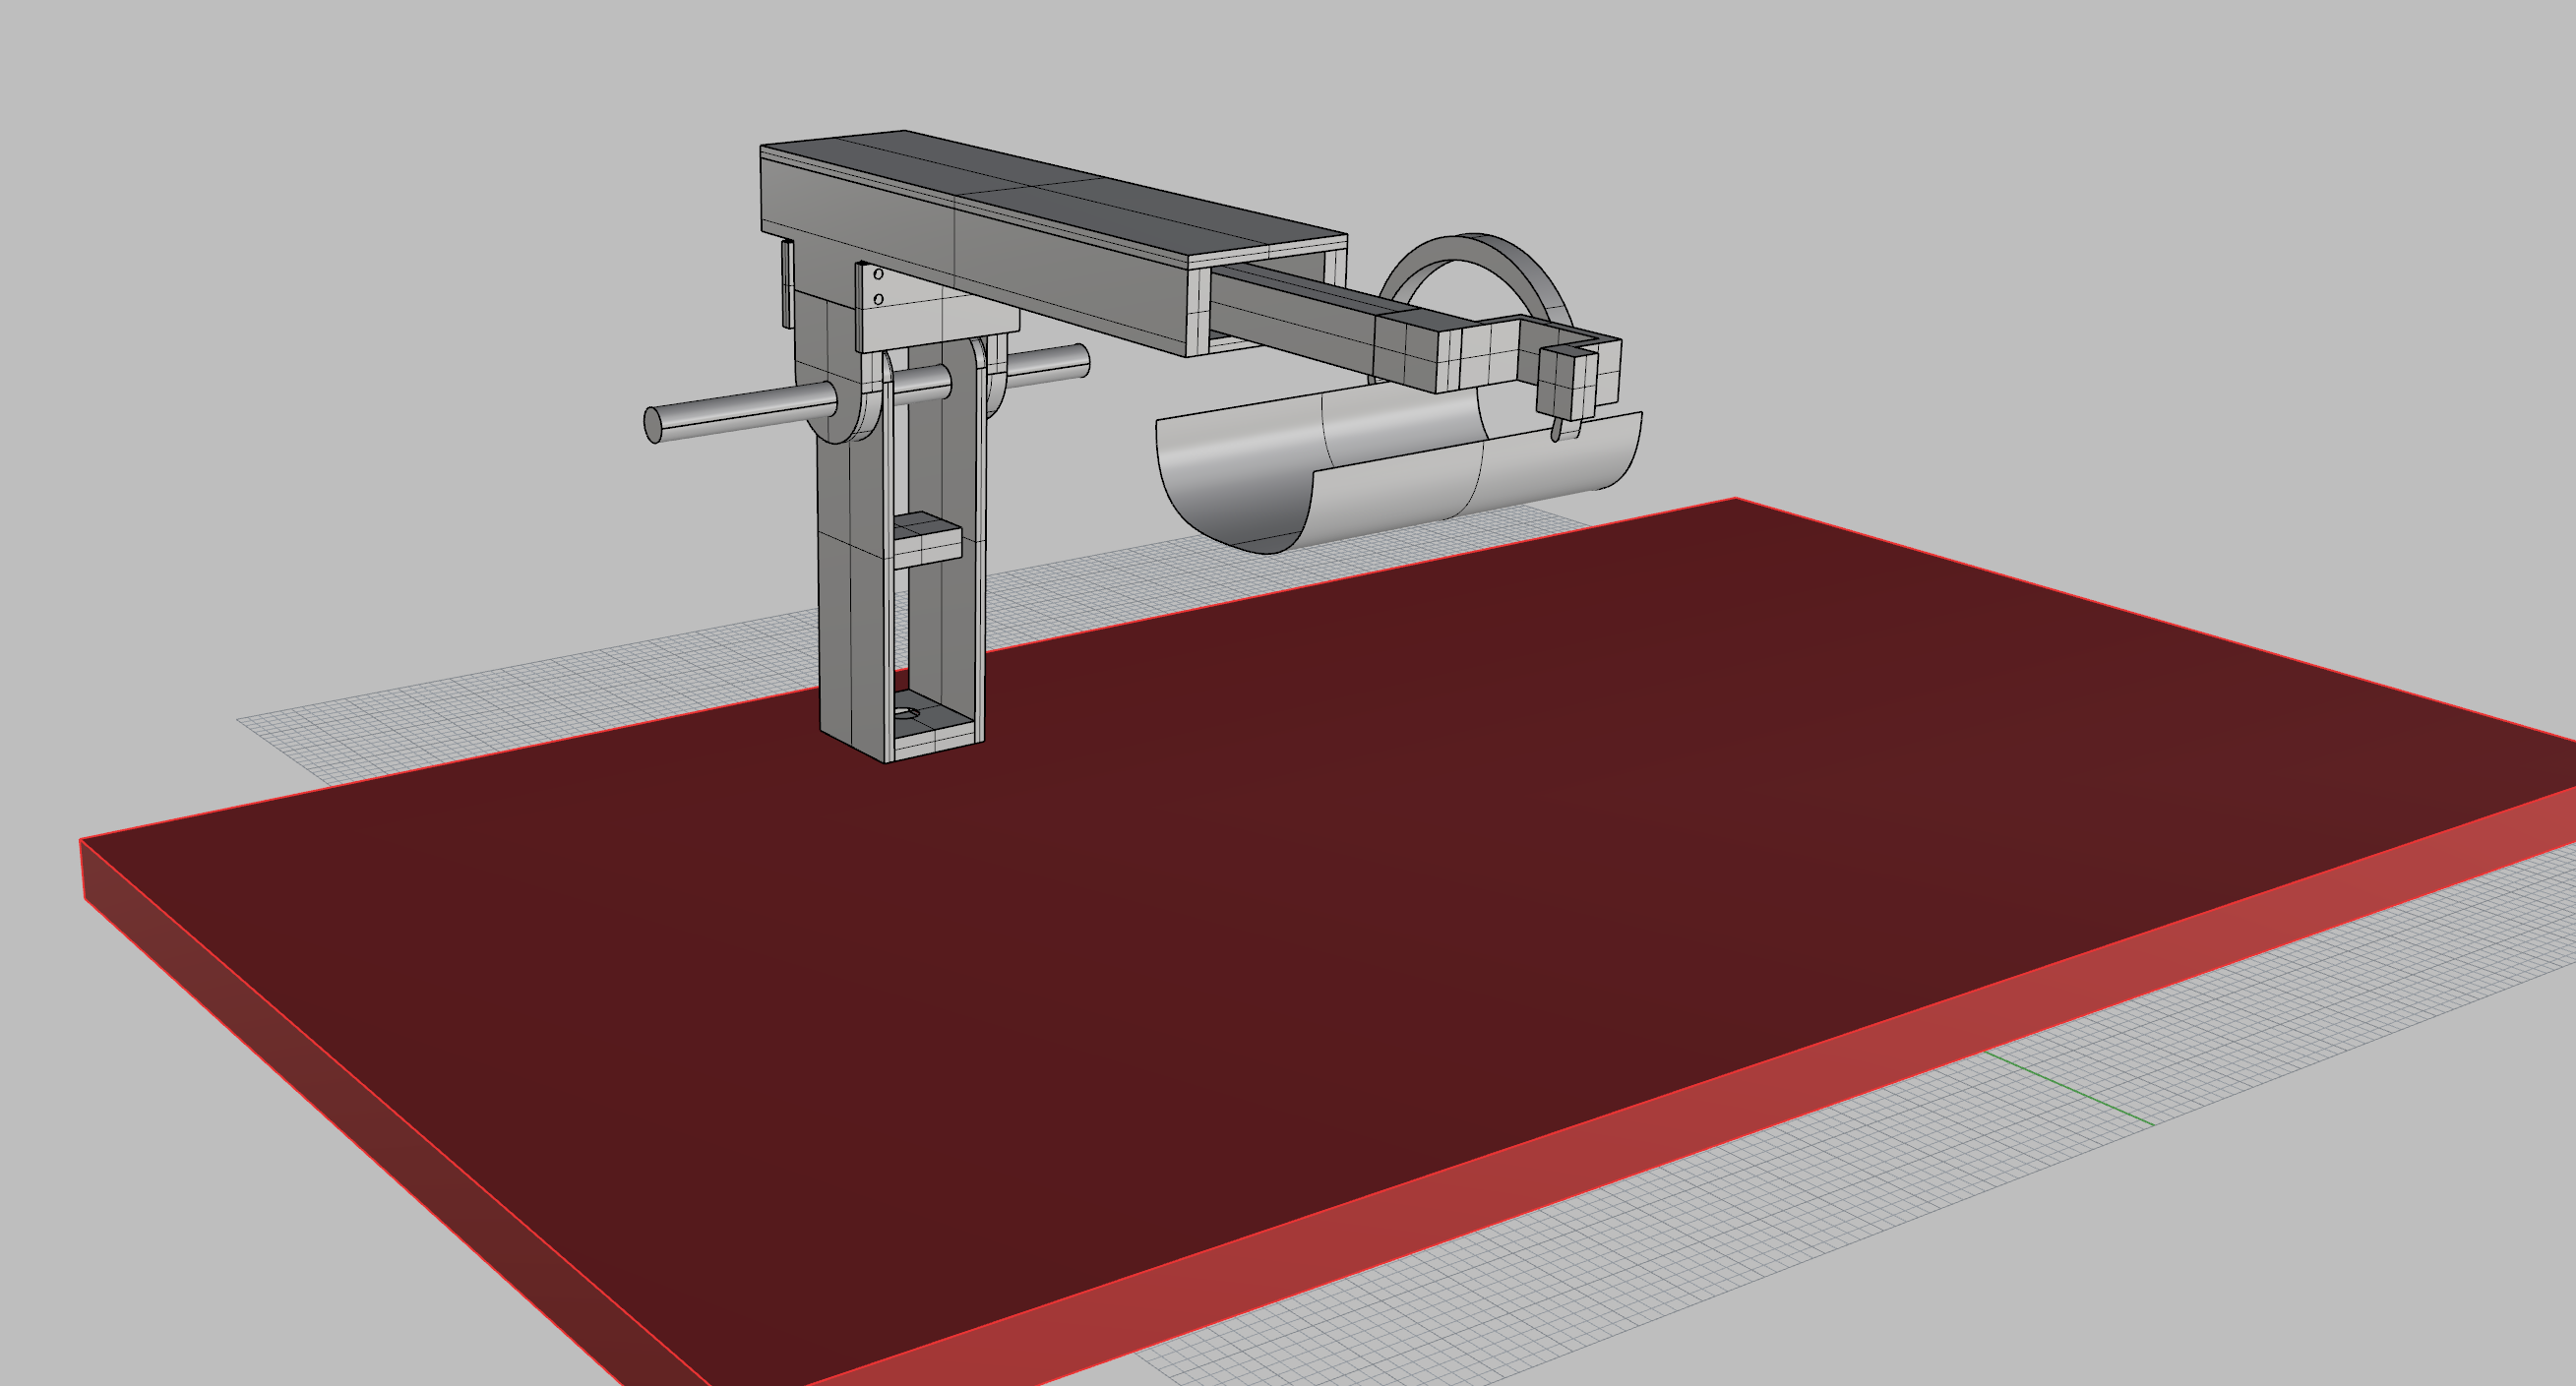
\includegraphics[width=\linewidth]{figures/ch3/bluedesign1}
	\caption{Figure showing the First proposed design of B.L.U.E.}
	\label{fig:blue1}
\end{figure}

\begin{figure}[p]%blue design 2
	\centering
	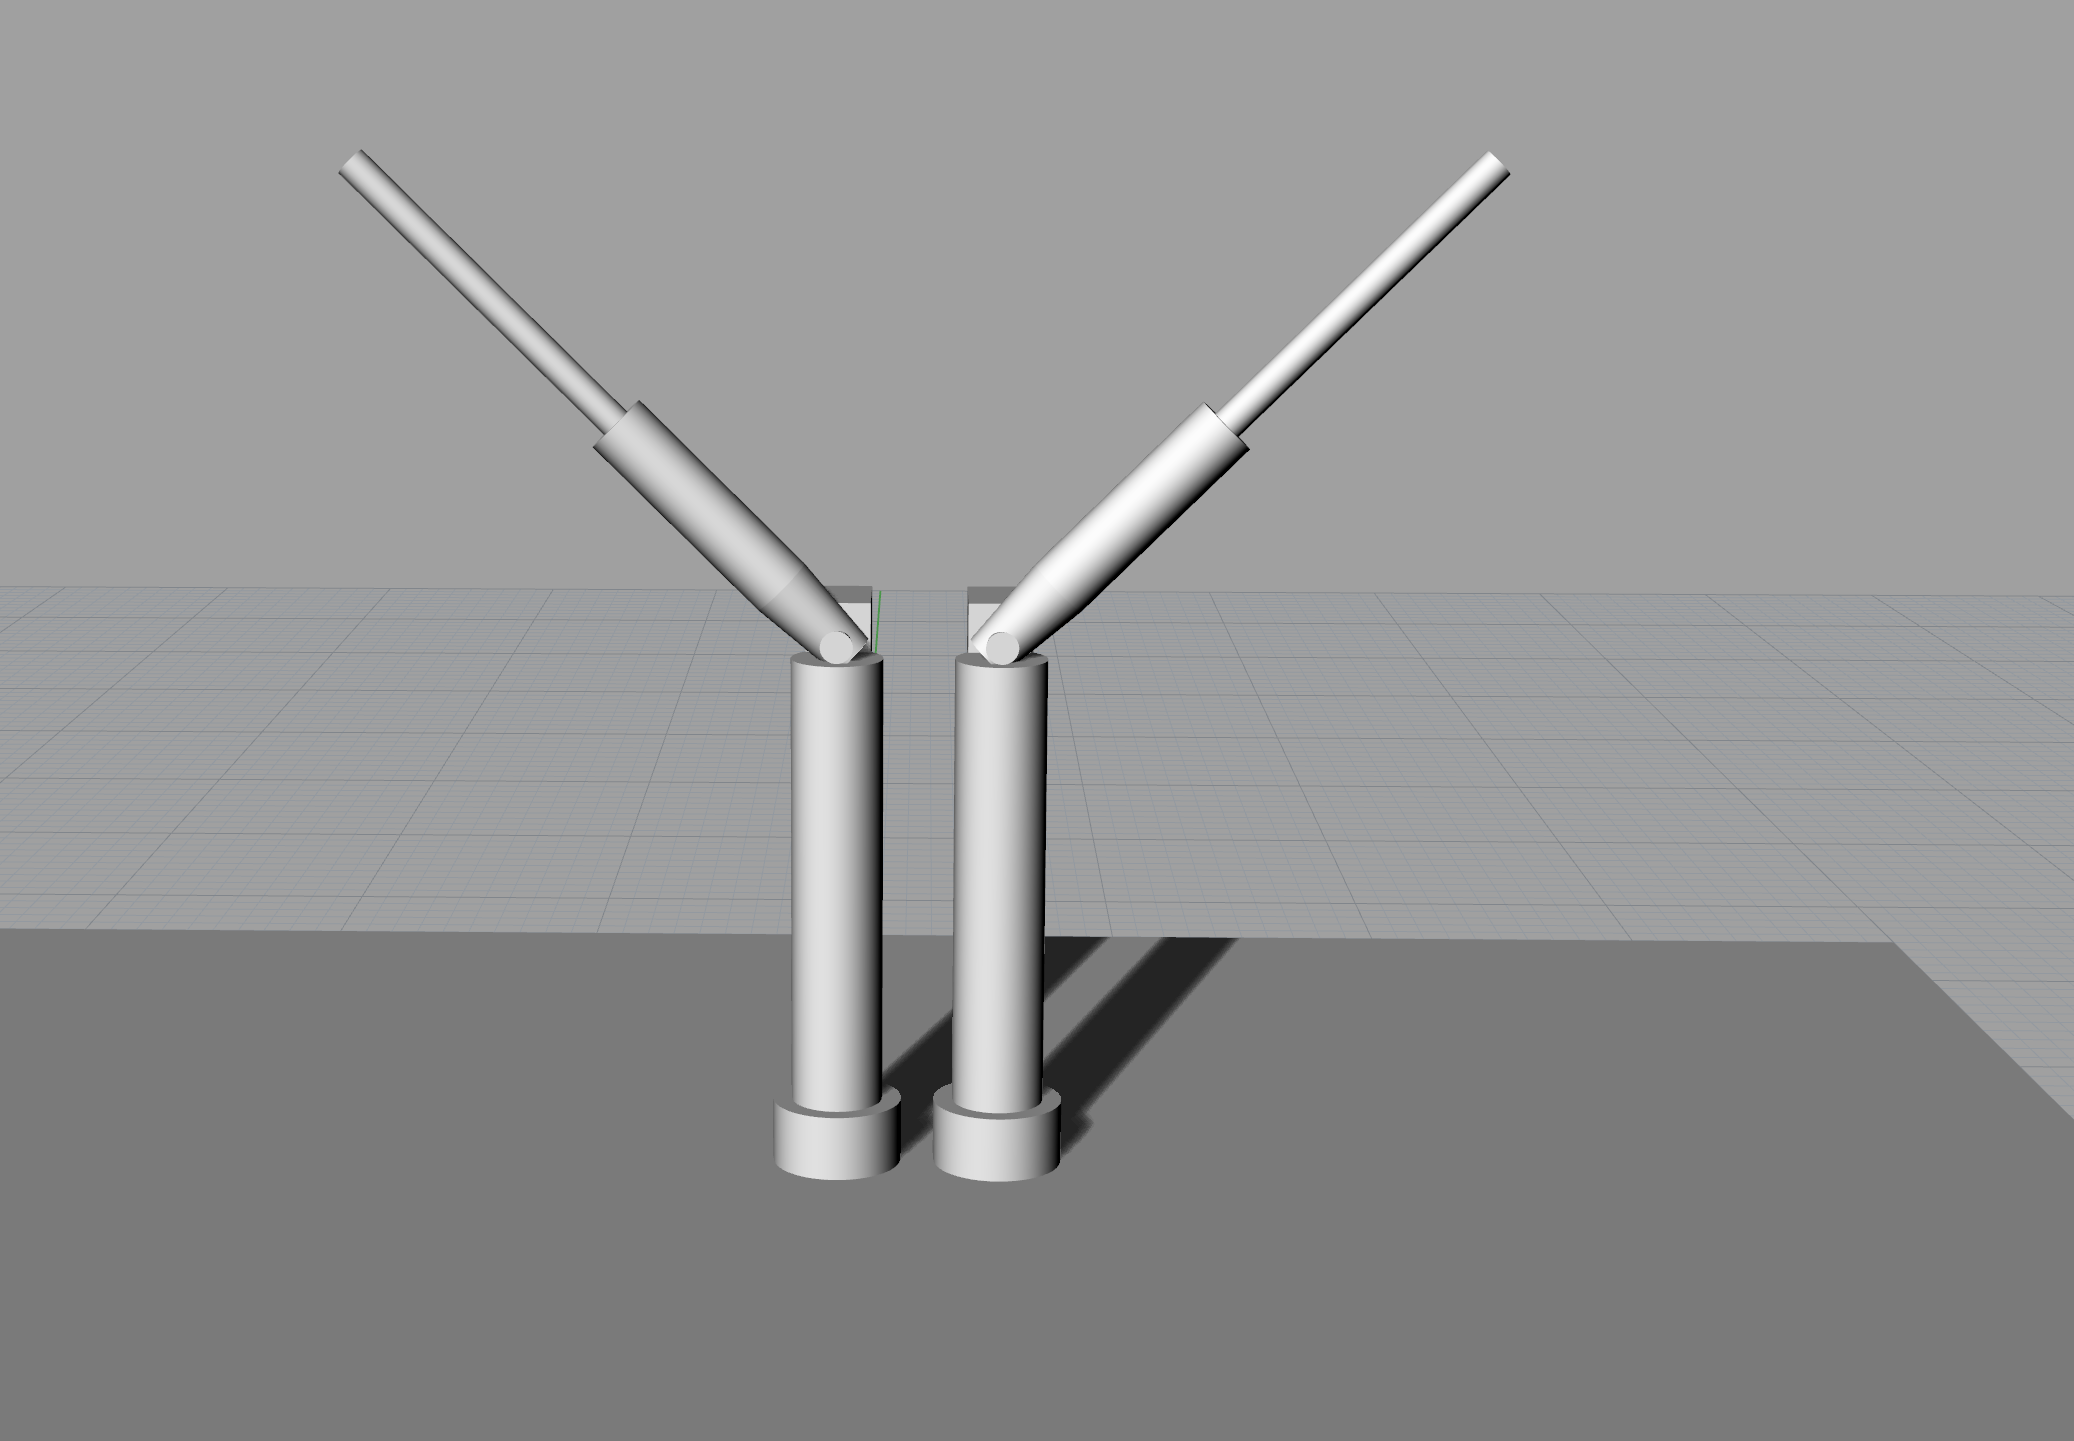
\includegraphics[width=\linewidth]{figures/ch3/bluedesign2}
	\caption{Figure showing the second proposed design of B.L.U.E.}
	\label{fig:blue2}
\end{figure}

\begin{figure}[p]%blue design 3
	\centering
	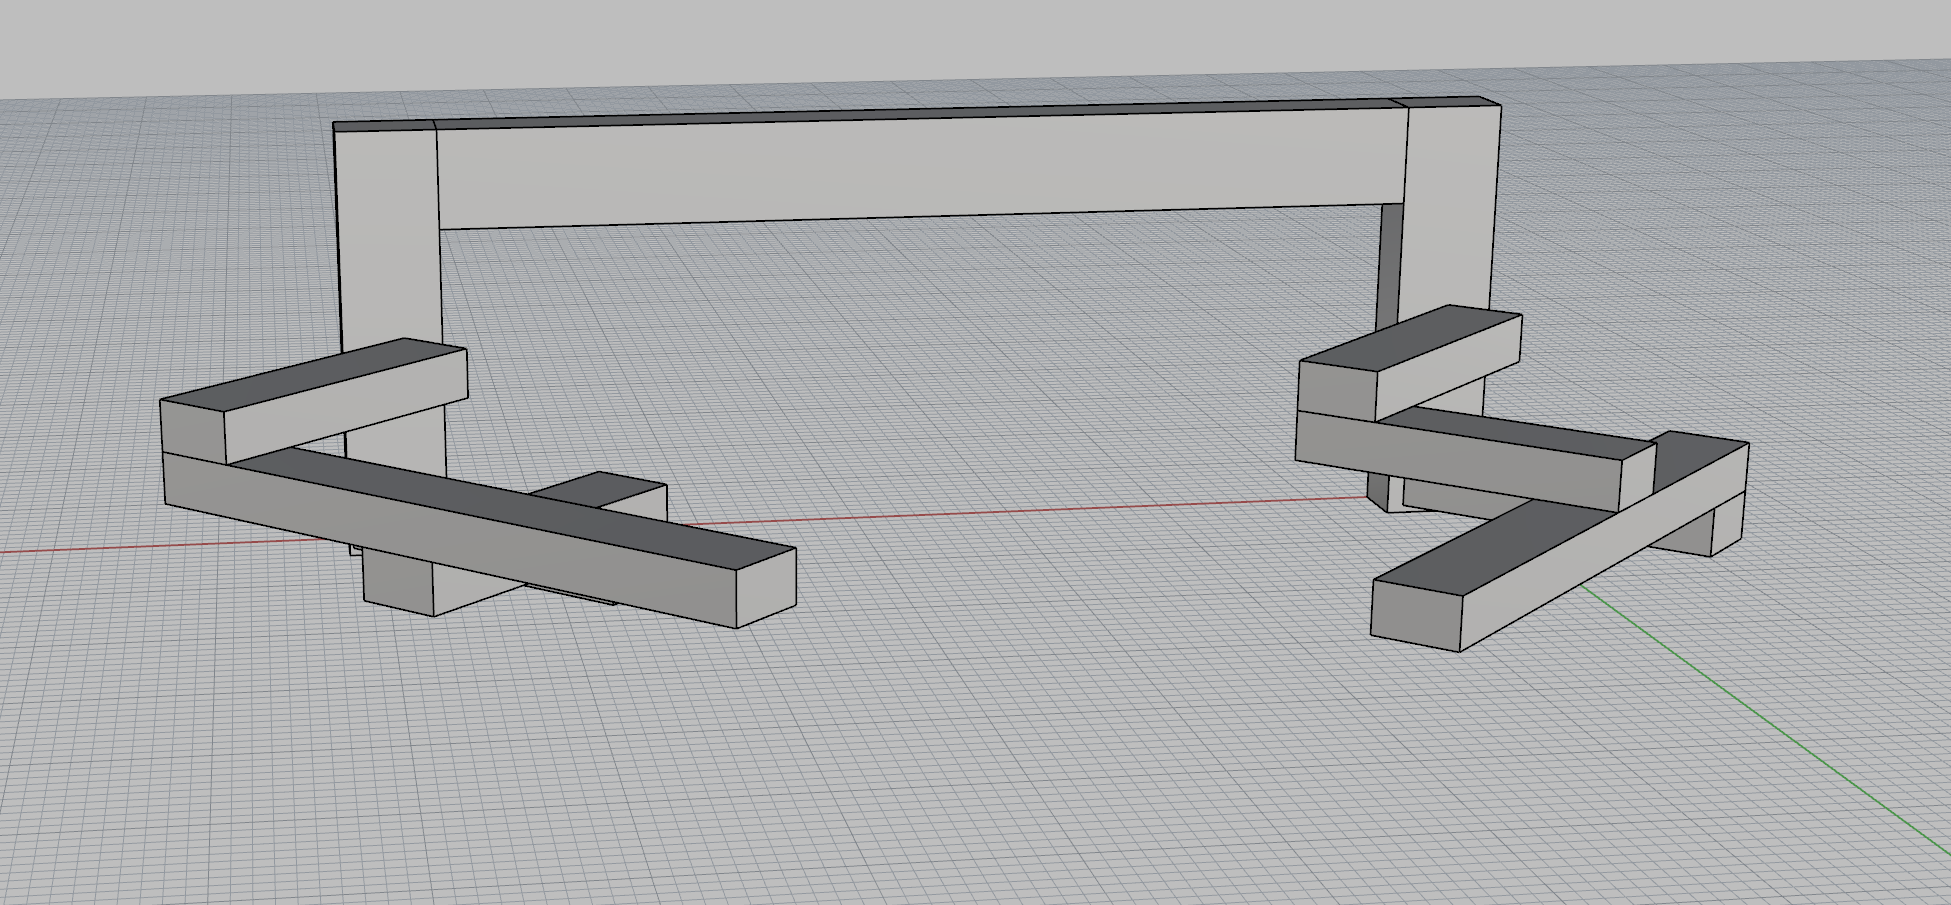
\includegraphics[width=\linewidth]{figures/ch3/bluedesign3}
	\caption{Figure showing the third proposed design of B.L.U.E.}
	\label{fig:blue3}
\end{figure}
\begin{figure}[p]%blue design presentation
	\centering
	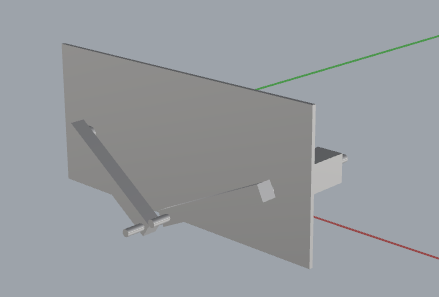
\includegraphics[width=\linewidth]{figures/ch3/bluepres}
	\caption{Figure showing the proposed Design for demonstration}
	\label{fig:bluepres}
\end{figure}
\subsection{Development of the \ac{blue} prototype}
The \ac{blue} prototype was developed as a means to show a visual representation of both a bilateral robot in action and a representation of a bilateral rehabilitation task.\\
The design used for the prototype based off the Driver's Seat robot \cite{Johnson1999,Johnson2003}, which brought about the design shown in Figure: \ref{fig:bluepres}. The materials chosen for implementation are 2 motors, 1 rotary encoder, 2 shafts with handle connectors and the control block.\\
For control of the system, a combination of both the bilateral active-passive control mode and the master-slave control mode explained in \ref{list:scontrol}, which involves a active mode on one of the motors, which will move an arm, and the master slave is implement through the rotary encoder to read the movements and tell the second motor to move in the other direction, the code to implement this is shown in the listing \ref{code:arduinomaster}.
\newpage

\section{Development of the Cascaded Force-Torque Sensor}\label{sec:forcesens}
\subsection{Design Process of the Force-Torque Sensor}
Designs on using a single-axis load cell to create a multi-axis structure had already been done in the research group before, with the result of this research producing a structure made in the design shown in Figure \ref{fig:loadcell1}.\\
Using the design above as a reference, I was able to come up with a design that measures forces in all the Cartesian axes shown in Figure \ref{fig:3dlc}. After the square brackets were made a change to the initial design was made due to the manufacturing of the load cells which meant not one of the load cells would be placed lower. The structure is design so as to behave like the commercial multi-axis force sensor shown in Figure:\ref{fig:3dlc}.\\
For the data from the load cells to be collected it is connected to a HX711 amplifier that is then connected to an arduino using the circuit connection as recommended from instructables \cite{Degraw2017} shown in Figure \ref{fig:sparkfun}, but replicated 3 times for this project.
\begin{figure}[p]%picture of assembly
	\centering
	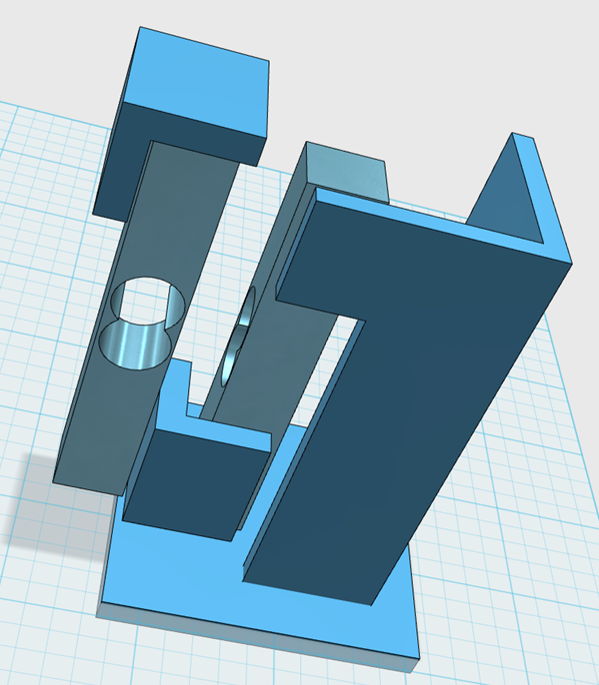
\includegraphics[width=\linewidth]{figures/ch3/loadcel1}
	\caption{Figure showing the completed assembly in testing}
	\label{fig:loadcell1}
\end{figure}

\begin{figure}[p]%forcesensorfigure
	\centering
	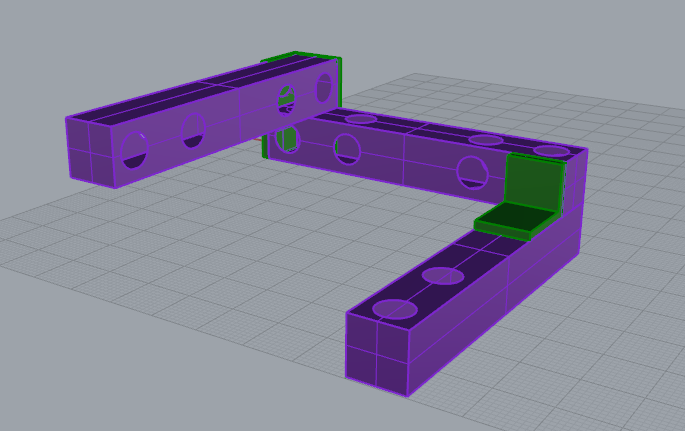
\includegraphics[width=\linewidth]{figures/ch3/loadcelldesign}
	\caption{Figure showing the first design for the 3-D force-Torque sensor}
	\label{fig:3dlc}
\end{figure}
\begin{figure}[p]%forcesensorfigure
	\centering
	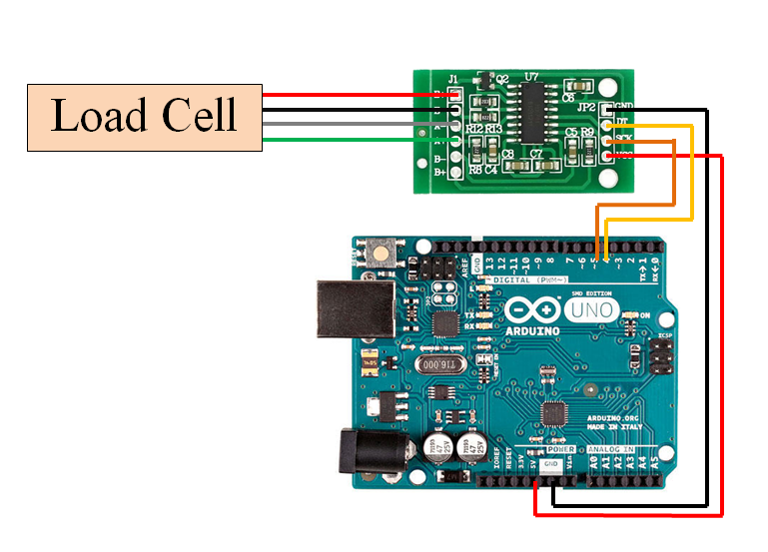
\includegraphics[width=\linewidth]{figures/ch3/sparkfun}
	\caption{Figure showing the Circuit diagram for using a commercial load cell with the HX711 amplifier \cite{Degraw2017}}
	\label{fig:sparkfun}
\end{figure}

\newpage



\subsection{Software Interface and Data Collection}
Before the load cells can be used for force measurement it has to be calibrated, the process of calibration for this system is easy and it involves having a object of known mass to then correct the calibration value till the output from the arduino matches the mass used. using the calibration code from instructables \cite{Degraw2017} shown in \ref{code:calibration} and the procedure shown in Figure \ref{fig:calibration}. Then once the calibration values have been obtained which are 5kg:361640, 10kg:220000, they can then be used in the code to obtain data for processing from the load cells.\\
After the structure had been assembled as shown in Figure \ref{fig:loadcelltest}, there was now a need for a suitable code to read from all 3 load cells simultaneously to python, for use in a transfer learning algorithm. Therefore the pyserial library was used to read data sent to the serial port from arduino that contains the data from each axis sent every 200ms, and the arduino code that sends the data to the serial shown in \ref{code:arduino}, and the python code which receives the data and saves it to a csv file is shown in \ref{code:py}.

\begin{figure}[p]%calibration images
	\centering
	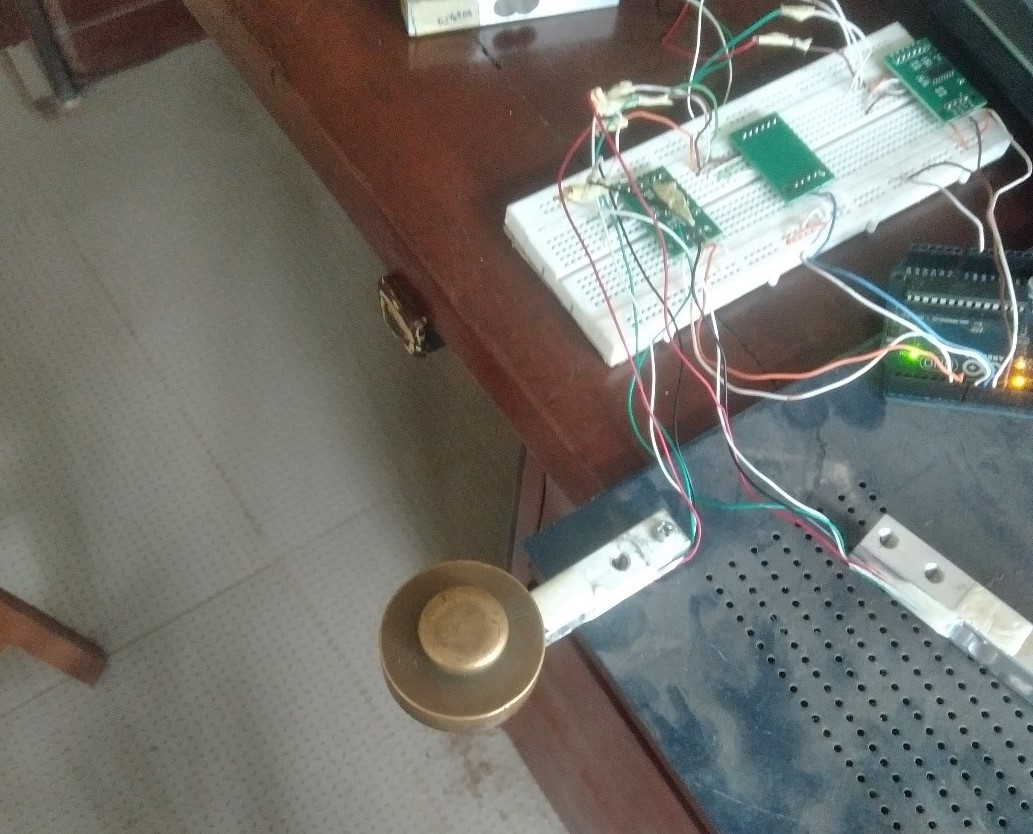
\includegraphics[width=15cm]{figures/ch3/calibration}
	\caption{Figure showing the calibration process}
	\label{fig:calibration}
\end{figure}

\begin{figure}[p]%picture of assembly
	\centering
	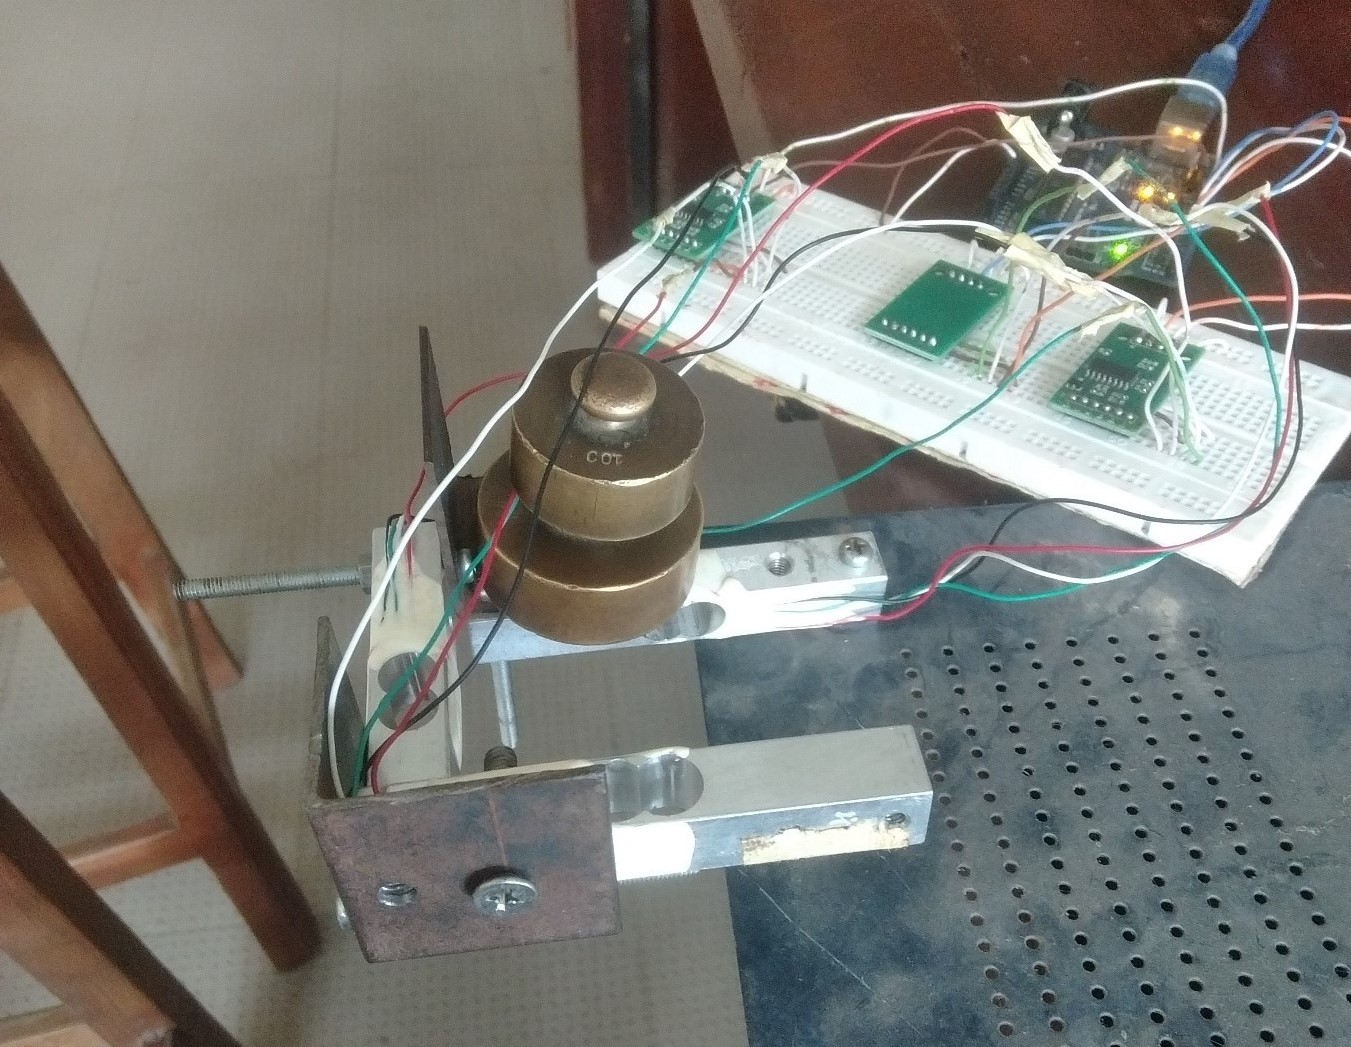
\includegraphics[width=\linewidth]{figures/ch3/loadcelltesting}
	\caption{Figure showing the completed assembly in testing}
	\label{fig:loadcelltest}
\end{figure}
\newpage
\subsection{Experiment Design and Implementation}\label{sec:experiment}
After the construction of the assembly had been completed, there is now a need to perform an experiment to confirm if the data from the novel multi-axis load cell from this study has worse prediction than a commercial multi-axis force sensor.\\
The concept of the design is to record the data from both force-sensors when the same force is applied to them both, but due to complications only data from the novel force-sensor was available for use. After the novel force sensor is assembled as it will be used, a range of force are applied to it at the end-effector point with varying magnitudes and force directions, to see the influence on the other load cells in the array, the experiment process is shown in Figure \ref{fig:loadcelltest}. The results of the test are shown in the next chapter.
%\subsection{Transfer Learning Problem Statement}
